\section*{1.1}
実数表示で$E_1=A_1\cos(kz-\omega t+\theta_1)$及び$E_2=A_2\cos(kz-\omega t+\theta_2)$と表される2つの光電場について,
\begin{enumerate}
    \renewcommand{\labelenumi}{(\alph{enumi})}
    \item 各光電場の振幅を複素表示で表せ.
    \item $E_1+E_2$の複素振幅を$E=Ae^{i\theta}$と表記した時の$A$及び$\theta$を$A_1,A_2,\theta_1,\theta_2$で表せ.
    \item 上記合成波$E$の光強度を$A_1,A_2,\theta_1,\theta_2$で表せ.但し,$光強度=|複素振幅|^2$とする.
\end{enumerate}

\subsection*{解答}
\begin{enumerate}
    \renewcommand{\labelenumi}{(\alph{enumi})}
    \item 各光電場の振幅の複素表示を$\tilde{A_1},\tilde{A_2}$とおくと
          \begin{eqnarray*}
            \tilde{A_1}=A_1e^{i\theta_1}\\
            \tilde{A_2}=A_2e^{i\theta_2}
          \end{eqnarray*}
    \item $E_1=A_1\cos(kz-\omega t+\theta_1)$,$E_2=A_2\cos(kz-\omega t+\theta_2)$より
          \begin{eqnarray*}
            E_1+E_2&=&A_1\cos(kz-wt+\theta_1)+A_2\cos(kz-wt+\theta_2)\\
            &=&A_1\{\cos(kz-wt)\cos\theta_1-\sin(kz-wt)\sin\theta_1\}+A_2\{\cos(kz-wt)\cos\theta_2-\sin(kz-wt)\sin\theta_2\}\\
            &=&(A_1\cos\theta_1+A_2\cos\theta_2)\cos(kz-wt)-(A_1\sin\theta_1+A_2\sin\theta_2)\sin(kz-wt)
          \end{eqnarray*}
          $E_1+E_2$の複素数表示を$\tilde{E}$とすると
          \begin{displaymath}
            \tilde{E}=\{A_1\cos\theta_1+A_2\cos\theta_2+i(A_1\sin\theta_1+A_2\sin\theta_2)\}e^{i(kz-wt)}
          \end{displaymath}
          よって
          \begin{eqnarray*}
            A&=&\{(A_1\cos\theta_1+A_2\cos\theta_2)^2+(A_1\sin\theta_1+A_2\sin\theta_2)^2\}^{\frac{1}{2}}\\
            &=&\{A_1^2+A_2^2+2A_1A_2(\cos\theta_1\cos\theta_2+\sin\theta_1\sin\theta_2)\}^{\frac{1}{2}}\\
            &=&\{A_1^2+A_2^2+2A_1A_2\cos(\theta_1-\theta_2)\}^{\frac{1}{2}}\\
          \end{eqnarray*}
          \begin{displaymath}
            \theta=tan^{-1}{\frac{A_1\sin\theta_1+A_2\sin\theta_2}{A_1\cos\theta_1+A_2\cos\theta_2}}
          \end{displaymath}
    \item 光強度を$I$とおくと
          \begin{displaymath}
            I=A^2=A_1^2+A_2^2+2A_1A_2\cos(\theta_1-\theta_2)
          \end{displaymath}
\end{enumerate}

\section*{1.2}
進行方向に対し垂直な$xy$平面上で,下左図のように,長辺と短辺の長さの比が$a:b$である長方形に接する楕円に沿って時計廻りで振動しながら伝播する強度$I_0$の平面波がある.
\begin{enumerate}
    \renewcommand{\labelenumi}{(\alph{enumi})}
    \item この光の偏波状態を上記パラメータを使った2次元ベクトルで表せ.
    \item 上記の光を$x$軸に対して角度$\theta$の直線振動成分のみを透過させる光素子(検光子)に通した.検光子透過後の光振幅を表せ.
    \item 透過光の強度を表せ.
    \item 透過光の偏波状態を$\{x,y\}$座標系(2次元ベクトル)で表せ.
\end{enumerate}

\begin{figure}[H]
    \begin{center}
        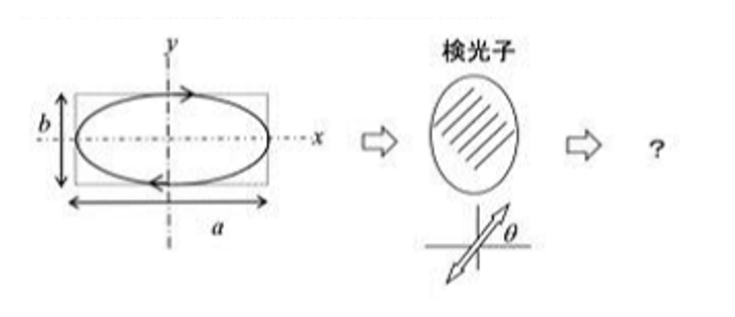
\includegraphics[width=100mm]{./figures/section/figure_1.eps}
    \end{center}
\end{figure}

\subsection*{解答}
\begin{enumerate}
    \renewcommand{\labelenumi}{(\alph{enumi})}
    \item $光強度=|複素振幅|^2$より\par
          $x$方向の複素振幅を$A_x$,$y$方向の複素振幅を$A_y$とすると
          \begin{displaymath}
            I_0=|A_x|^2+|A_y|^2
          \end{displaymath}
          また
          \begin{displaymath}
            A_x:A_y=a:b
          \end{displaymath}
          よって
          \begin{eqnarray*}
            I_0&=&|A_x|^2+\frac{b^2}{a^2}|A_y|^2\\
            &=&\frac{a^2+b^2}{a^2}|A_x|^2
          \end{eqnarray*}
          ゆえに
          \begin{eqnarray*}
            A_x=\frac{a\sqrt{I_0}}{\sqrt{a^2+b^2}}\\
            A_y=\frac{b\sqrt{I_0}}{\sqrt{a^2+b^2}}
          \end{eqnarray*}
          右廻り楕円偏波なので,求める偏波状態は
          \begin{displaymath}
            E=\left(\frac{a\sqrt{I_0}}{\sqrt{a^2+b^2}}, A_y=\frac{b\sqrt{I_0}}{\sqrt{a^2+b^2}}e^{-\frac{\pi}{2}i}\right)
          \end{displaymath}
    \item 光の強度が$I_0$より振幅は$\sqrt{I_0}$なので検光子透過後の光振幅は
          \begin{displaymath}
            \sqrt{I_0}\cos\theta
          \end{displaymath}
    \item 透過光の強度は
          \begin{displaymath}
            I_0\cos^2\theta
          \end{displaymath}
    \item 透過光の偏波状態は
          \begin{displaymath}
            \left(\frac{\sqrt{I_0}}{\sqrt{a^2+b^2}}a\cos\theta, \frac{\sqrt{I_0}}{\sqrt{a^2+b^2}}b\cos(\frac{\pi}{2}-\theta)\right)
          \end{displaymath}
\end{enumerate}

\section*{1.3}
右斜め45度の直線偏光波を$x/y$方向振動成分に対する屈折率がそれぞれ$n_x/n_y$である長さ$L$の複屈折媒質に入射したところ,出射光の偏波状態が,光波長が$\lambda_1$の時には左斜め直線,$\lambda_2$の時には左廻り円偏波,であった.
$\lambda_1$と$\lambda_2$の関係を上記パラメータを用いて表せ.
但し,媒質長は偏波状態が元に戻るほどには長くないものとする.

\begin{figure}[H]
    \begin{center}
        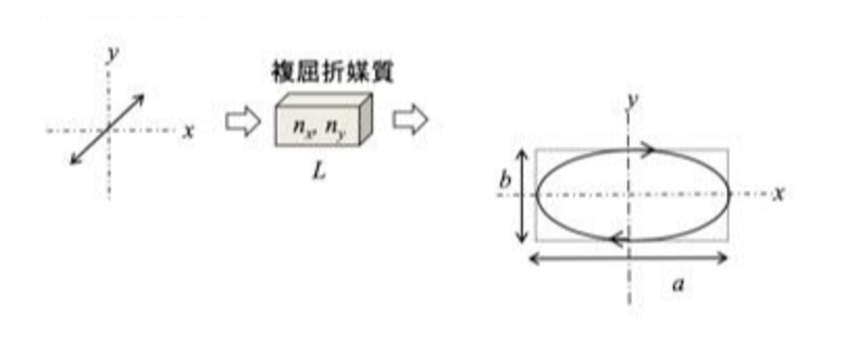
\includegraphics[width=100mm]{./figures/section/figure_2.eps}
    \end{center}
\end{figure}

\subsection*{解答}
\noindent
右斜め45度の直線偏光波の偏波状態は$(A_x, A_y)e^{-i\omega t}$
複屈折媒質透過後の偏波状態は
\begin{eqnarray*}
  (A_xe^{in_xk_0L}, A_ye^{in_yk_0L})e^{-i\omega t}\\
  =(A_x, A_ye^i{n_y-n_x}k_0L)e^{in_xk_0L}e^{-i\omega t}
\end{eqnarray*}
ただし,$k_0=\frac{2\pi}{\lambda}$
$\lambda=\lambda_1$のとき左斜め直線になることから
\begin{eqnarray*}
  e^{i(n_y-n_x)k_0L}=e^{i\pi}\\
  (n_y-n_x)k_0L=\pi\\
  k_0=\pi\frac{L}{n_y-n_x}\\
  \frac{2\pi}{\lambda_1}=\pi\frac{1}{(n_y-n_x)L}\\
  \lambda_1=2(n_y-n_x)L
\end{eqnarray*}
$\lambda=\lambda_2$のとき左廻り円偏波になるので
\begin{eqnarray*}
  e^{i(n_y-n_x)k_0L}=e^{i\frac{\pi}{2}}\\
  (n_y-n_x)k_0L=\frac{\pi}{2}
\end{eqnarray*}
先ほどと同様にして
\begin{displaymath}
  \lambda_2=4(n_y-n_x)L
\end{displaymath}
よって$\lambda_1=\frac{1}{2}\lambda_2$